\documentclass[12pt]{article}
\usepackage[utf8]{inputenc} % Suporte a caracteres UTF-8
\usepackage{graphicx} % Suporte para inserir imagens
\usepackage[hidelinks]{hyperref}% Links e URLs
\usepackage{amsmath} % Fórmulas matemáticas


\title{
\textbf{
    Documento de Requisitos  \\
    \vspace{4cm}\huge Projeto ProfScore\vspace{2cm}
}}

\author{
    Carlos Henrique Cruz Xavier \\
    Guilherme Vasconcelos Horita \\ 
    Leonardo Sousa Ferreira Fadul \\ 
    \vspace{4cm}
}
\date{\today}

\begin{document}

\maketitle

\newpage % Quebra de página para o conteúdo principal
\tableofcontents  % Gera o sumário automaticamente

\newpage % Quebra de página para o conteúdo principal
\section{Introdução}
Aqui você descreve o contexto do projeto.

\subsection{Propósito do documento de requisitos}
\hspace{1cm} O objetivo do projeto é criar um aplicativo que permita a avaliação dos
professores universitários pelos alunos da UNIFEI. Este projeto destina-se aos
alunos da Universidade Federal de Itajubá que estão em período de matrícula
nas disciplinas.

\subsection{Escopo do produto}
\hspace{1cm} O produto é um aplicativo que permite aos alunos da UNIFEI avaliar os professores com base em critérios pré-definidos, como metodologia, clareza, assiduidade, e outros aspectos relevantes. O aplicativo fornecerá relatórios de avaliação que poderão ser usados pela universidade para aprimorar o processo de ensino. O produto não incluirá funcionalidades como matrícula de alunos, gestão de notas, ou integração com outros sistemas acadêmicos.

\subsection{Definições, acrônimos e abreviações}
\begin{center}
\begin{tabular}{|c|l|}
\hline
\textbf{Sigla/Termo} & \textbf{Significado} \\
\hline
App & Aplicativo móvel ou web \\
\hline
DR & Documento de Requisitos \\
\hline
ProfScore & Professor Score \\
\hline
UNIFEI & Universidade Federal de Itajubá \\
\hline
Usuário & Aluno de universidade que utiliza o aplicativo \\
\hline
\end{tabular}
\end{center}


\subsection{Referências}
\begin{itemize}
    \item IEEE Std 830-1998: IEEE Recommended Practice for Software Requirements Specifications.
    \item  Artigo “Best Practices in Software Requirement Specifications”, John
Doe, 2022, Journal of Software Engineering.
\end{itemize}

\subsection{Visão geral do documento de requisitos}
você descreve o contexto do projeto.
\begin{itemize}
    \item  Descrição Geral - Fornece uma visão geral do sistema, incluindo suas funcionalidades principais e restrições.
    \item  Requisitos Específicos - Detalha os requisitos funcionais e não funcionais do sistema.
    \item  Modelos e Diagramação - Apresenta diagramas de casos de uso, sequência e outros relevantes.
\end{itemize}


\section{Descrição Geral}
Liste os objetivos principais do sistema.
\subsection{Perspectiva do Produto}
\begin{itemize}
    \item \textbf{Usuário:} Alunos avaliam professores; administradores acessam relatórios detalhados.
    \item \textbf{Hardware:} Acessível por dispositivos desktop e móveis; hospedado em servidores robustos.
    \item \textbf{Software:} Frontend com React e Styled-Components; Backend com Node.js e Express; Banco de Dados PostgreSQL com Prisma ORM.
    \item \textbf{Comunicação:} API RESTful para interação entre frontend e backend; notificações para usuários;
\end{itemize}
\subsection{Funções do Produto}
\hspace{1cm} As principais funções são mostrar para o usuario o rankiong dos professores e suas avaliacoes.
\subsection{Características do Usuário}
\hspace{1cm}Usuarios sao alunos da unfei com idade +- 18 a 30 anos.
\subsection{Restrições}
\hspace{1cm} O software não será integrado com o sistema da UNIFEI.
\subsection{Suposições e Dependências}
\begin{itemize}
    \item Sistema Linux 
    \item Sistema Linux 
\end{itemize}

\section{Requisitos Específicos}
\subsection{Requisitos Não Funcionais}
    \subsubsection{RNF01 - Desempenho}
        O sistema deve ser capaz de suportar simultaneamente pelo menos 1.000 usuários ativos sem degradação significativa de desempenho.
    \subsubsection{RNF02 - Segurança}
        Todos os dados sensíveis devem ser criptografados tanto em trânsito quanto em repouso para garantir a segurança e a privacidade das informações dos usuários.
    \subsubsection{RNF04 - Usabilidade}
        O aplicativo deve ter uma interface intuitiva e responsiva, garantindo uma experiência de usuário satisfatória em dispositivos desktop e móveis.
    \subsubsection{RNF05 - Manutenibilidade}
        O código deve ser modular e bem documentado, facilitando a manutenção e a adição de novas funcionalidades.
\subsection{ Interfaces Externas}
\subsection{Requisitos Funcionais}
    \subsubsection{RF01 - Cadastro de Usuário}
        O sistema deve permitir o cadastro de novos usuários (alunos e administradores) com informações básicas como nome, e-mail e senha.
    \subsubsection{RF02 - Login e Autenticação}
        O sistema deve fornecer um mecanismo de autenticação seguro para que os usuários possam acessar o aplicativo com suas credenciais.
    \subsubsection{RF03 - Avaliação de Professores}
        Os alunos devem poder avaliar professores com base em critérios pré-definidos, como metodologia, clareza, assiduidade, etc.
    \subsubsection{RF04 - Visualização de Avaliações}
         Os alunos devem poder visualizar suas avaliações submetidas e o status atual das mesmas.
    \subsubsection{RF05 - Relatórios para Administradores}
        O sistema deve gerar relatórios detalhados das avaliações para os administradores da universidade, permitindo a análise das métricas.
    \subsubsection{RF06 - Gestão de Perfis}
        Usuários (alunos e administradores) devem poder atualizar suas informações de perfil, como e-mail e senha.
    \subsubsection{RF07 - Notificações}
        O sistema deve enviar notificações aos usuários sobre o status de suas avaliações e relatórios disponíveis.
    \subsubsection{RF08 - Filtro e Pesquisa de Professores}
        O sistema deve permitir que os alunos filtrem e pesquisem professores com base em critérios como departamento, nome e disciplinas lecionadas.
    \subsubsection{RF09 - Histórico de Avaliações}
        O sistema deve manter um histórico das avaliações realizadas por cada aluno, permitindo que eles revisitem e editem avaliações anteriores, se necessário, dentro de um período definido.
    \subsubsection{RF10 - Feedback e Sugestões}
        O sistema deve fornecer uma opção para que os alunos deixem feedback adicional e sugestões sobre os professores, além dos critérios de avaliação padrão. Este feedback será enviado para revisão e possível inclusão nos relatórios administrativos.

\subsection{Requisitos Lógicos de Banco de Dados}
\subsection{Restrições de Projeto}
\subsection{Atributos do Sistema de Software}


\newpage
\section{Diagramas}
\subsection{Caso de Uso}
\begin{figure}[h]
\centering
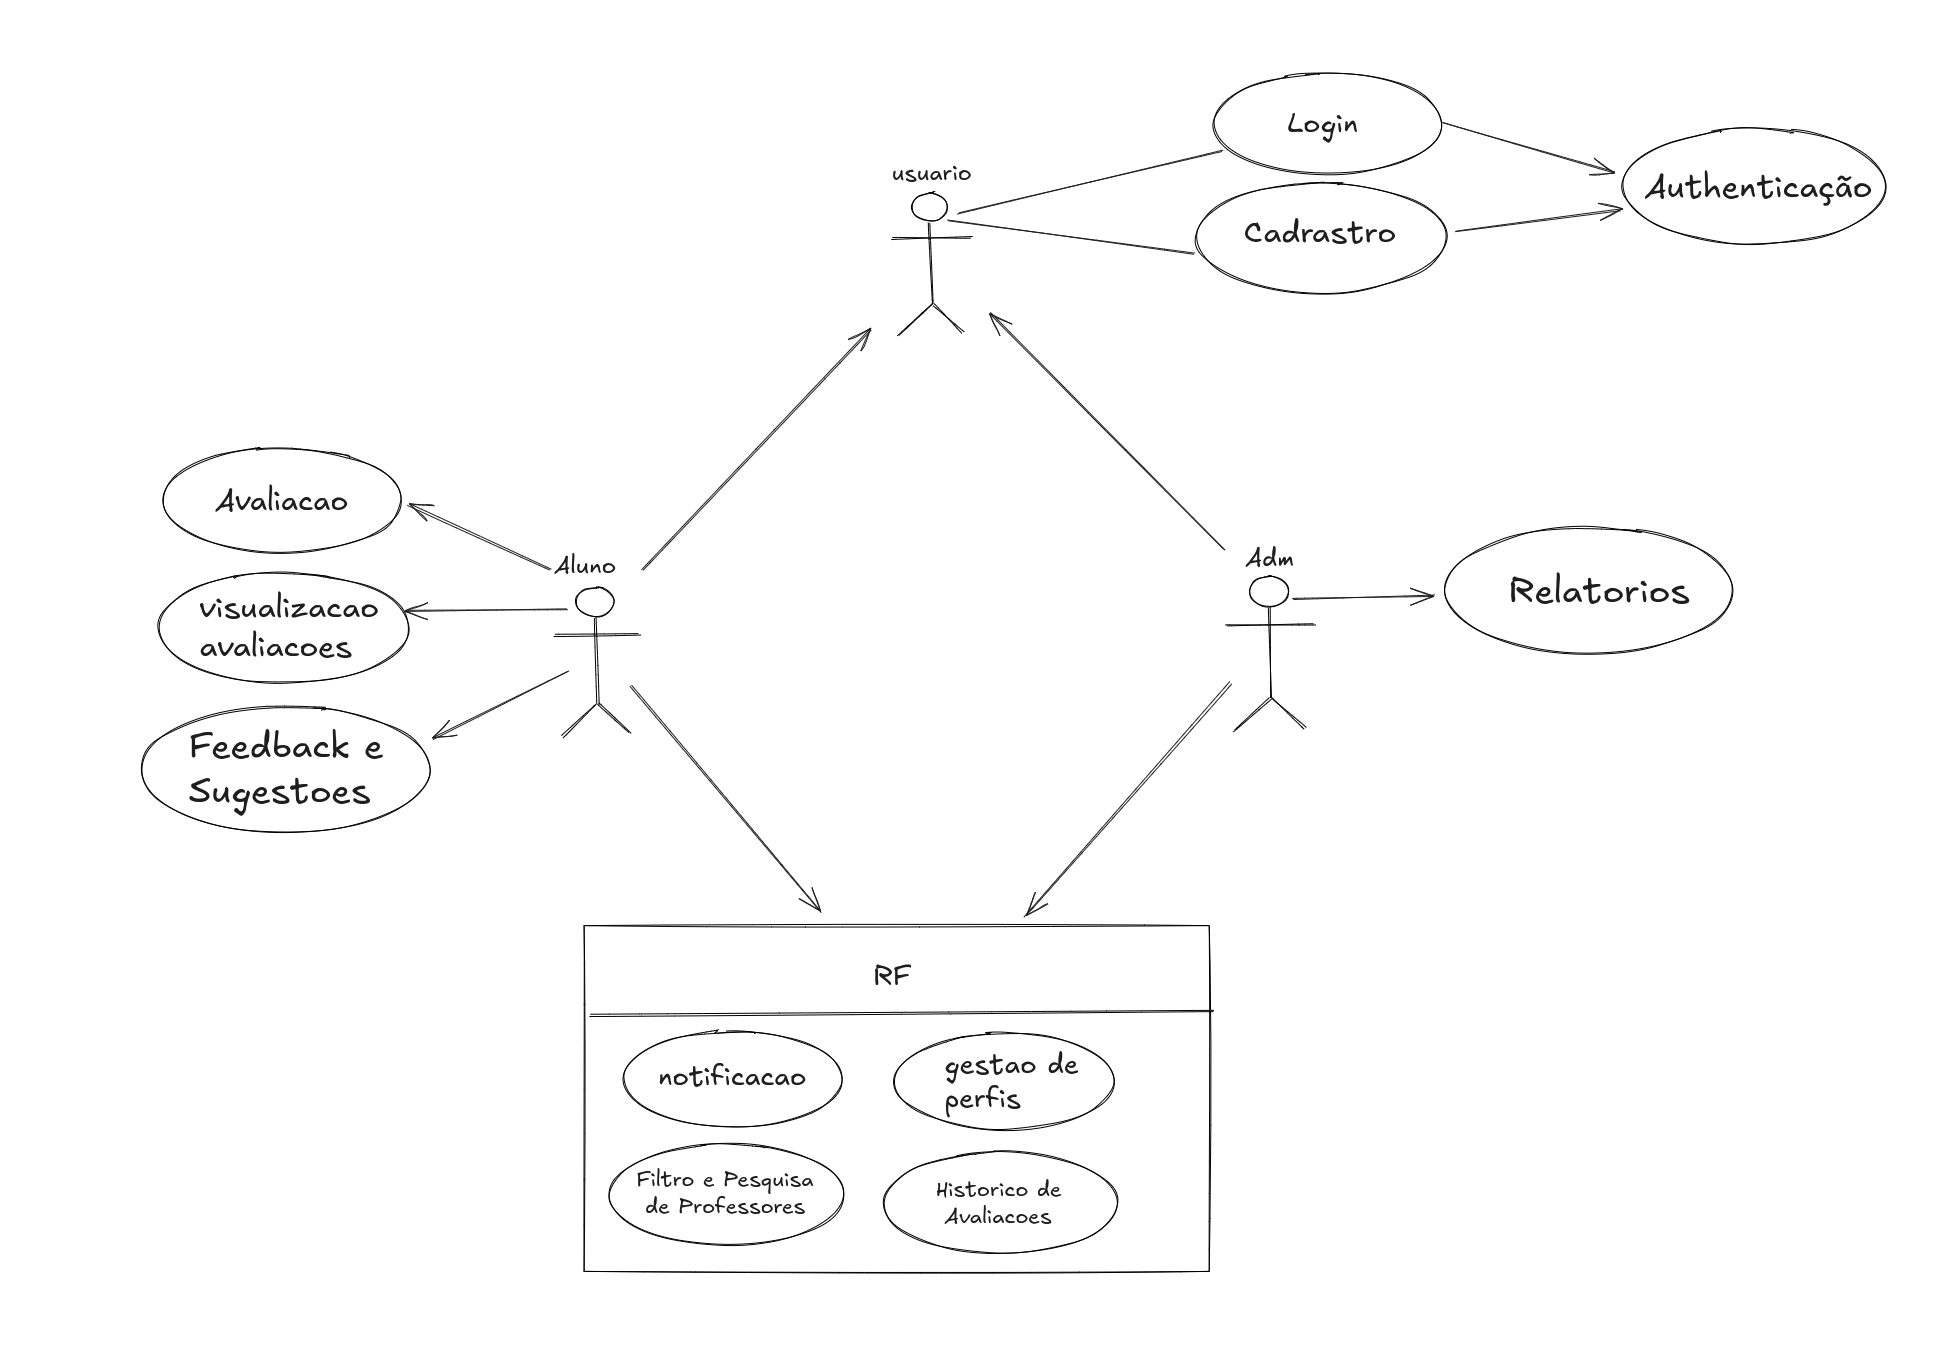
\includegraphics[width=1\textwidth]{useCaseProfScore.png} % Insere uma imagem chamada diagrama.png
\caption{Diagramas Caso de Uso}
\end{figure}
\clearpage
\subsection{Interação}
\begin{figure}[h]
\centering
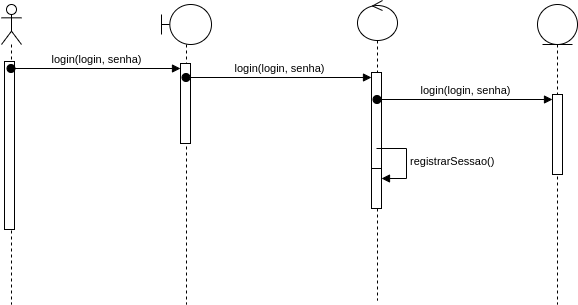
\includegraphics[width=1\textwidth]{diagramaInteracao.drawio.png} % Insere uma imagem chamada diagrama.png
\caption{Diagramas Caso de Uso}
\end{figure}


\section{Conclusão}
Conclusão do documento.

\end{document}
